\documentclass[a4paper]{article}
\newif\ifshowcode
\showcodetrue

\usepackage{latexsym}
\usepackage[portuges]{babel}
\usepackage{a4wide}
\usepackage[utf8]{inputenc}
\usepackage{graphicx}
\usepackage{graphics}
\usepackage{glossary}
\usepackage{algorithmic}
\usepackage{algorithm}
\usepackage{listings}

\parindent=0pt
\parskip=2pt

\setlength{\oddsidemargin}{0in}
\setlength{\evensidemargin}{0in}
\setlength{\topmargin}{0in}
\addtolength{\topmargin}{-\headheight}
\addtolength{\topmargin}{-\headsep}
\setlength{\textheight}{8.9in}
\setlength{\textwidth}{6.5in}
\setlength{\marginparwidth}{0.5in}

%
% Report to Engineering Languages UCE
%
\title{\huge  \\ \bigskip
\begin{figure}[!ht]
\begin{center}

\includegraphics[width=0.2\textwidth]{./Images/um-eng.jpg}
\end{center}
\end{figure}
{\small Universidade do Minho}\\
{\vspace{2cm} \Huge \textbf{XBOOK}}\\
{\vspace{1cm} \large Mestrado de Informática, Engenharia de Linguagens}\\
{\large Processamento Estruturado de Documentos}\\
}
\date{\vspace{4cm} \LARGE \textbf{20 de Fevereiro de 2009}}
\author{\large Sérgio Areias pg$º$13381 \and \large Hugo Areias pg$º$11060}

\makeglossary

\storeglosentry{glos:XML}{name={XML}, description={Extensible Markup Language}}
\storeglosentry{glos:PDF}{name={PDF}, description={Portable Document Format}}
\storeglosentry{glos:CSS}{name={CSS}, description={Cascading Style Sheets}}
\storeglosentry{glos:XSL}{name={XSL}, description={Extensible Stylesheet Language}}
\storeglosentry{glos:HTML}{name={HTML}, description={HyperText Markup Language}}

\begin{document}
\pagenumbering{roman}
\maketitle
\newpage
\large \tableofcontents
\pagenumbering{arabic}

\newpage
%%
% Secção - Introdução
%%
\section{\LARGE Introdução}

\hspace{1cm}Tendo em conta que uma grande quantidade de informação começa a ser disponibilizada em formato digital, incluíndo livros, a forma como esta é apresentada e as ferramentas que nos permitem atingir esses objectivos, de uma forma rápida e pouco complexa, começam a ser importantes.

\hspace{1cm}Neste projecto vamos tentar fazer algo objectivo para o problema em questão já que qualquer coisa genérica tende também a ser muito complexa, ou seja, vamos focar-nos numa amostra mais pequena e depois se possível tentar fazer com que se este se aproxime de algo mais no meio-termo, nem muito específico (limita o seu uso) nem muito genérico.

\hspace{1cm}Vamos dividir este relatório em quatro problemas. O primeiro a construção do \verb|schema| em que nos vamos basear para implementar o segundo e o terceiro problema, ou seja, a conversão de {\em XML}\useglosentry{glos:XML} para {\em PDF}\useglosentry{glos:PDF} e o gerar de uma página {\em HTML}\useglosentry{glos:HTML} com o conteúdo do documento.

\hspace{1cm}O quarto problema baseia-se na implementação de um editor para ser mais fácil e intuitiva a alteração dos documentos {\em XML}\useglosentry{glos:XML} baseados no nosso \verb|schema|

\hspace{1cm}Este projecto foi desenvolvido com o auxílio às ferramentas \verb|Oxygen|\footnote{{\em http://www.oxygenXML.com/}}, para criar o nosso projecto, e \verb|latex|\footnote{{\em http://www.latex-project.org/}}, para gerar o este relatório.\\

\newpage
%%
% Secção - Descrição do Problema
%%
\section{\LARGE Descrição do Problema}

  %%
  % Secção
  %%
\subsection{\large Breve Introdução ao Problema}

\hspace{1cm}Neste projecto, que nós escolhemos dentro de um variado leque de alternativas, é nos proposto desenvolver uma aplicação em {\em XML}\useglosentry{glos:XML} para suporte à criação de livros.

\hspace{1cm}Já existem aplicações deste tipo, mas normalmente são muito genéricas (por exemplo o {\em DocBook}\footnote{{\em http://www.docbook.org/tdg/en/HTML/docbook.HTML}} que é utilizado pela {\em O'Reilly}\footnote{{\em http://oreilly.com/}}) e tendem a ser muito complexas, por isso a ideia será desenvolver um que possa ser usado como suporte às disciplinas do nosso departamento.

\hspace{1cm}Além da criação de uma {\em stylesheet}, usando {\em CSS}\useglosentry{glos:CSS} e {\em XSL}\useglosentry{glos:XSL}, para fazer a conversão de {\em XML}\useglosentry{glos:XML} para {\em PDF}\useglosentry{glos:PDF}, tivemos também que desenhar uma {\em stylesheet} para fazer a conversão para páginas {\em HTML}\useglosentry{glos:HTML} e criar um editor para fácil manipulação do conteúdo do {\em Xbook}.\\

  %%
  % Secção
  %%
\subsection{Objectivos a Cumprir}

A realização deste projecto envolve as seguintes etapas:\\

\begin{itemize}
\item "Especificação do schema: o Xbook deverá tomar como referência o conteúdo do livro de apoio à disciplina para a especificação do schema: site do livro."
\item "Tranformação para PDF: deverão ser seguidas as formatações especificadas no template Word da FCA: template."
\item "Transformação para HTML: fica ao seu critério."
\item "Interface de Edição: deverá ser desenvolvida uma interface de edição para o Authentic."
\item "Elaboração do relatório final: o relatório final deverá ser elaborada em XML e deverá estar de acordo com o Schema fornecido pelo docente e que foi discutido com os alunos nas aulas."
\end{itemize}

\newpage

%%
% Secção
%%
\section{\LARGE Schema}

\subsection{\large Designação dos Elementos}
                               
\bigskip
\begin{center}
\begin{tabular}[c]{|l|l|l|l|}
\hline
\large\textbf{Elemento} & \large\textbf{Designação} & \large\textbf{Elemento} & \large\textbf{Designação}\\
\hline
\normalsize xbook & \normalsize Elemento raíz & \normalsize table & \normalsize Tabela\\
\hline
\normalsize metainfo & \normalsize Informação sobre o livro & \normalsize hline & \normalsize Linha de uma tabela\\
\hline
\normalsize preface & \normalsize Prefácio & \normalsize cell & \normalsize Célula de uma tabela\\
\hline
\normalsize intro & \normalsize Introdução & \normalsize header & \normalsize Cabeçalho de uma tabela\\
\hline
\normalsize body & \normalsize Corpo do livro & \normalsize define & \normalsize Definições\\
\hline
\normalsize conclusion & \normalsize Conclusão & \normalsize itemize & \normalsize Listas não numeradas\\
\hline
\normalsize rec_reads & \normalsize Leituras Recomendadas & \normalsize item & \normalsize Elemento de uma lista não numerada\\
\hline
\normalsize exercises & \normalsize Exercícios & \normalsize enumeration & \normalsize Lista numerada\\
\hline
\normalsize appendix & \normalsize Apêndice & \normalsize enum & \normalsize Elemento de uma lista numerada\\
\hline
\normalsize glossary & \normalsize Glossário & \normalsize example & \normalsize Exemplo\\
\hline
\normalsize index & \normalsize Index & \normalsize ex & \normalsize Componentes do exemplo\\
\hline
\normalsize bibliography & \normalsize Bibliografia & \normalsize fig & \normalsize Figura\\
\hline
\normalsize chapter & \normalsize Capítulo & \normalsize img & \normalsize Caminho para uma imagem\\
\hline
\normalsize section & \normalsize Secção & \normalsize caption & \normalsize Legenda de uma tabela ou figura\\
\hline
\normalsize subsection & \normalsize Subsecção & \normalsize code & \normalsize Bloco de código\\
\hline
\normalsize entry & \normalsize Entrada da bibliografia & \normalsize comment & \normalsize Documentação de codigo\\
\hline
\normalsize summary & \normalsize Sumário do Capítulo & \normalsize note & \normalsize Nota\\
\hline 
\normalsize exercise & \normalsize Uma alínea de exercício & \normalsize italic & \normalsize Itálico\\
\hline
\normalsize title & \normalsize Título & \normalsize bold & \normalsize Negrito\\
\hline
\normalsize subtitle & \normalsize Subtítulo & \normalsize super & \normalsize Sobre a linha\\
\hline
\normalsize frontcover & \normalsize Imagem da capa do livro & \normalsize sub & \normalsize Sob a linha\\
\hline
\normalsize authors & \normalsize Lista de autores & \normalsize strike & \normalsize Rasurado\\
\hline 
\normalsize author & \normalsize Informação sobre um autor & \normalsize under & \normalsize Sublinhado\\
\hline
\normalsize local & \normalsize Localidade & \normalsize equation & \normalsize Fórmula matemática\\
\hline
\normalsize publisher & \normalsize Editora & \normalsize term & \normalsize Termo\\
\hline
\normalsize date & \normalsize Data de edição do livro & \normalsize obs & \normalsize Observação\\
\hline
\normalsize name & \normalsize Nome & \normalsize exp & \normalsize Expressão\\
\hline            
\normalsize email & \normalsize Contacto e-mail do autor & \normalsize citation & \normalsize Citação\\
\hline
\normalsize id & \normalsize Número de identificação do autor & \normalsize year & \normalsize Ano de edição\\
\hline
\normalsize degree & \normalsize Grau académico & \normalsize url & \normalsize Caminho para uma página externa\\
\hline
\normalsize rank & \normalsize Cargo na empresa & \normalsize figref & \normalsize Referência para uma figura\\
\hline
\normalsize affiliation & \normalsize Empresa afiliada & \normalsize tabref & \normalsize Referência para uma tabela\\
\hline
\normalsize webpage & \normalsize Página pessoal & \normalsize chpref & \normalsize Referência para um capítulo\\
\hline   
\normalsize photo & \normalsize Foto do autor & \normalsize secref & \normalsize Referência para uma secção\\
\hline 
\normalsize textblock & \normalsize Bloco de componentes complexos & \normalsize exref & \normalsize Referência para um exemplo\\
\hline
\normalsize paragraph & \normalsize Bloco de texto & \normalsize  & \normalsize  \\
\hline   
\end{tabular}
\end{center}

\newpage

\subsection{\large Principais Decisões}
              
\hspace{1cm}A estrutura do \verb|schema| foi desenvolvida de modo a fornecer uma boa legibilidade dos diferentes elementos ao utilizador, facilitando também a compreensão da linguagem e consequentemente uma maior facilidade em manter o \verb|schema|. Todos os elementos que compôem a linguagem \emph{XBook} encontram-se ao mesmo nível na visualização do \verb|schema| sendo utilizadas referências quando necessitamos de embutir algum elemento dentro de outro elemento. Com esta decisão o \verb|schema| fica devidamente organizado facilitando a procura e o acesso a qualquer elemento do mesmo. Ao nível da estrutura tomamos uma outra decisão que afectou significativamente o resultado final das várias \emph{stylesheets}. Decidimos manter os elementos "inúteis" que podiam ser facilmente eliminados do \verb|schema|, isto é, mantivemos elementos que poderiam ser agregados noutro elemento ou até eliminados, por exemplo, os elementos \emph{webpage} e \emph{url} são ambos ligações ao exterior, logo poderiam ser agregados no mesmo elemento. No nosso caso isso não ocorre porque uma \emph{webpage} é similar a uma \emph{url}, mas nós queremos manter a diferenciação de diferentes elementos, ou seja, uma \emph{webpage} é na realidade uma \emph{url} mas o contrário não se verifica, logo o elemento \emph{webpage} será definido como uma referência para o elemento \emph{url} visto que faz parte do universo das \emph{urls}. Estes casos ocorrem várias vezes no \verb|schema| do \emph{XBook} daí que este seja um pouco complexo quando se têm em vista criar uma instância do mesmo. Outro exemplo um pouco diferente é o caso do parágrafo que é um conjunto de formatações de texto misturadas com o próprio texto. Este elemento poderia ser eliminado e o conteúdo dele replicado pelos vários elementos que o utilizam, isto não iria afectar o funcionamento da linguagem mas aumentaria a complexidade do código, o tamanho do \verb|schema| e a redundância de elementos, visto que se iria substituir o elemento parágrafo por todos os elementos que o compôem actualmente.

\hspace{1cm}Os índices gerados no documento \emph{PDF}\useglosentry{glos:PDF} e nas páginas \emph{HTML}\useglosentry{glos:HTML} não aparecem directamente especificados no \verb|schema|, devido ao facto de não ser necessário o auxílio do autor para criar os vários índices. Os índices são gerados automaticamente pelas \emph{stylesheets} sendo apenas requisitado ao autor que decida se lhe interessam a totalidade dos índices ou só apenas alguns na construção do seu livro. Os índices são seleccionados através de três atributos na raíz do
\emph{XBook} \emph{(toc,tof,tot)}, sendo o índice de conteúdos obrigatério e os restantes opcionais.

\hspace{1cm}Para a nossa linguagem criamos propositadamente dois tipos simples com o objectivo de, mais uma vez, aumentar o nível de legibilidade do \verb|schema| e ajudar a identificar o que o elemento ou atributo representa. Os tipos básicos são a \emph{label} e o \emph{text}, ou seja, associar etiquetas a elementos permitindo declarar referências para os mesmos e declarar o nosso próprio tipo de dados para texto. A criação desses tipos é apresentada de seguida:\\
          
\begin{small}
\begin{lstlisting}
<xs:simpleType name="label">
    <xs:restriction base="xs:string"/>
</xs:simpleType>
<xs:simpleType name="text">
    <xs:restriction base="xs:string"/>
</xs:simpleType>
\end{lstlisting}
\end{small}      

\hspace{1cm}Apesar destas decisões o nosso \verb|schema| poderia ainda ser melhorado em certos aspectos, frisando aqui alguns deles, como a adição de mais elementos possíveis de serem utilizados num livro, uma pequena evolução na definição de alguns elementos e a alteração da disposição de alguns elementos permitindo algumas melhorias nas \emph{stylesheets} ao nível da legibilidade e eficiência.\\

\subsection{\large Elementos Principais}

\hspace{1cm}Um livro, para se encontrar de acordo com a especificação do \emph{XBook}, necessita, para começar, de conter a meta-informação respectiva (título, autores, editora, etc.), seguida do prefácio, introdução, corpo do livro e conclusão. Estes elementos são obrigatérios em qualquer livro escrito em \emph{XBook} e são relativamente semelhantes, excepto o corpo do livro. Também são válidos os livros que contenham apíndice, glossário, bibliografia, leituras recomendadas, exercícios e index, mas todos estes elementos são opcionais não tendo necessariamente de aparecer num livro realizado na linguagem \emph{XBook}.

\hspace{1cm}Também nos elementos opcionais existem vários semelhantes aos anteriores, como o caso das leituras recomendadas e o apíndice que tem praticamente o mesmo comportamento quando processados pelas \emph{stylesheets}. A estrutura básica desses elementos é a seguinte:\\

\begin{small}
\begin{lstlisting}
<xs:element name=[name]>
    <xs:complexType>
        <xs:sequence>
            <xs:element ref="title"/>
            <xs:element ref="textblock"/>
        </xs:sequence>
    </xs:complexType>
</xs:element>
\end{lstlisting}
\end{small}

\hspace{1cm}Claro está que nem todos os elementos são tão simples como o exemplo acima apresentado, alguns elementos contêm recursividade directa enquanto outros contêm indirecta. As subsecções são um exemplo de um elemento com recursividade directa, porque uma subsecção pode conter várias subsecções no seu conteúdo.\\

\begin{small}
\begin{lstlisting}
<xs:element name="subsection">
    <xs:complexType>
        <xs:sequence>
            <xs:element ref="title"/>
            <xs:element ref="textblock"/>
            <xs:element minOccurs="0" maxOccurs="unbounded" ref="subsection"/>
        </xs:sequence>
        <xs:attribute name="label" type="label" use="required"/>
    </xs:complexType>
</xs:element>
\end{lstlisting}
\begin{center}
\begin{footnotesize}
\caption{Exemplo de recursividade directa}
\end{footnotesize}
\end{center}
\end{small}

Por outro lado as listas não numeradas são elementos que utilizam recursividade indirecta, o que faz com que seja mais difícil implementar o seu comportamento nas \emph{stylesheets}.\\

\begin{small}
\begin{lstlisting}
<xs:element name="itemize">
    <xs:complexType>
        <xs:sequence maxOccurs="unbounded">
            <xs:element ref="item"/>
        </xs:sequence>
    </xs:complexType>
</xs:element>

<xs:element name="item">
    <xs:complexType>
        <xs:choice>
            <xs:element ref="paragraph"/>
            <xs:element ref="define"/>
            <xs:element ref="itemize"/>
            <xs:element ref="enumeration"/>
        </xs:choice>
    </xs:complexType>
</xs:element>
\end{lstlisting}
\begin{center}
\begin{footnotesize}
\caption{Exemplo de recursividade indirecta}
\end{footnotesize}
\end{center}
\end{small}

\hspace{1cm}Para finalizar, os dois elementos mais importantes para a elaboração dos textos e inserção de qualquer outro tipo de informação são o bloco de texto e o parágrafo. O parágrafo está contido no bloco de texto, e permite a inserção dos tipos básicos de formatação de texto e alguns tipos especiais, para além do texto elaborado pelo autor. O bloco de texto engloba o parágrafo e os restantes tipos complexos, como as tabelas, figuras, etc. Ambas as implementações são apresentadas de seguida.\\

\begin{small}
\begin{lstlisting}
<xs:element name="paragraph">
    <xs:complexType mixed="true">
        <xs:choice maxOccurs="unbounded" minOccurs="0">
            <xs:element ref="italic"/>
            <xs:element ref="bold"/>
            <xs:element ref="super"/>
            <xs:element ref="sub"/>
            <xs:element ref="strike"/>
            <xs:element ref="term"/>
            <xs:element ref="under"/>
            <xs:element ref="exp"/>
            <xs:element ref="citation"/>
            <xs:element ref="year"/>
            <xs:element ref="url"/>
            <xs:element ref="figref"/>
            <xs:element ref="tabref"/>
            <xs:element ref="secref"/>
            <xs:element ref="chpref"/>
            <xs:element ref="exref"/>
            <xs:element ref="local"/>
            <xs:element ref="name"/>
        </xs:choice>
    </xs:complexType>
</xs:element>
\end{lstlisting}
\begin{center}
\begin{footnotesize}
\caption{Disposição do parágrafo no \verb|schema|}
\end{footnotesize}
\end{center}
\end{small}

\begin{small}
\begin{lstlisting}
<xs:element name="textblock">
    <xs:complexType mixed="true">
        <xs:choice maxOccurs="unbounded">
            <xs:element ref="paragraph"/>
            <xs:element ref="define"/>
            <xs:element ref="itemize"/>
            <xs:element ref="enumeration"/>
            <xs:element ref="subtitle"/>
            <xs:element ref="note"/>
            <xs:element ref="example"/>
            <xs:element ref="table"/>
            <xs:element ref="equation"/>
            <xs:element ref="obs"/>
            <xs:element ref="code"/>
            <xs:element ref="fig"/>
        </xs:choice>
    </xs:complexType>
</xs:element>
\end{lstlisting}
\begin{center}
\begin{footnotesize}
\caption{Disposição do bloco de texto no \verb|schema|}
\end{footnotesize}
\end{center}
\end{small}

\newpage

%%
% Secção
%%
\section{\LARGE Gerar PDF com XSL:FO}

\hspace{1cm}Para conseguirmos moldar a forma como é apresentado o conteúdo do livro, tivemos que criar vários formatos de páginas, por exemplo, para diferenciar as páginas pares das ímpares, ou para podermos ter a disposição do conteúdo das secções diferente da forma como apresentamos o índice, o prefácio, etc.

\hspace{1cm}Visto isto definimos um formato para a capa, um formato para os capítulos, outro para o conteúdo das secções e, por fim, um para todas as páginas não incluídas neste conjunto (prefácio, introdução, conlusão, etc.).\\

  %%
  % Secção
  %%

\subsection{\large Gerar a Capa do Livro}

\hspace{1cm}Para gerarmos o formato da capa, começamos por definir o tamanho da folha e o tamanho das margens que esta iria. Podemos ver abaixo o código que desenvolvemos para definir o formato que iria ter a capa.\\
  
\begin{small}
\begin{lstlisting}
  <fo:simple-page-master master-name="title-page" 
      page-width="210mm" page-height="297mm" margin-top="3cm"
      margin-bottom="3cm" margin-left="2cm" margin-right="2cm">
    <fo:region-body margin-top="0cm" margin-bottom="2cm" 
                    margin-left="1cm" margin-right="1cm"/>
    <fo:region-before extent="0.5cm"/>
    <fo:region-after extent="0.5cm" border-after-width="0.5cm"/>
    <fo:region-start extent="2cm"/>
    <fo:region-end extent="2cm"/>
  </fo:simple-page-master>
\end{lstlisting}
\end{small}

\hspace{1cm}Depois do formato já definido era então necessário preencher a capa dependendo da informação do livro que dispomos. Antes de tudo decidimos que o número de páginas tinham que ser pares (ou seja duas neste caso), para forçar uma página em branco logo a seguir à capa.\\

\begin{small}
\begin{lstlisting}
  <fo:page-sequence master-reference="title-page" force-page-count="even">
\end{lstlisting}
\end{small}
  
\hspace{1cm}Para respeitar as normas da FCA\footnote{{\em http://www.fca.pt/}}, a editora do livro é um campo obrigatório do \verb|schema| (como achamos que faz todo o sentido), e aparece no fundo de todas as páginas do livro. Vamos mostrar o código, que permite desenvolver esta propriedade do livro, neste tópico mesmo este sendo usado na definição de todas as outras secções do nosso livro.\\

\begin{small}
\begin{lstlisting}
    <fo:static-content flow-name="xsl-region-after">
      <fo:block font="7pt Copperplate Gothic Bold" text-align="center">
        <xsl:value-of select="metainfo/publisher"/>
      </fo:block>
    </fo:static-content>
\end{lstlisting}
\end{small}
    
\hspace{1cm}A imagem do livro poderia ter sido definida na região {\em xsl-region-before} mas, como obrigamos o número de páginas a ser par, então a imagem apareceria na segunda página que, supostamente tem que estar vazia. Poderiamos resolver este problema criando um novo formato para {\em blank pages}, passando a capa a ter só uma página logo seguida de uma página em branco.\\

\begin{small}
\begin{lstlisting}
    <fo:flow flow-name="xsl-region-body">
      <fo:block text-align="right" padding-bottom="2cm">
        <fo:external-graphic src="url('{metainfo/frontcover/img/@path}')" 
                                  content-height="50%"/>
\end{lstlisting}
\end{small}
  
\hspace{1cm}Para o resto da informação, o tratamento feito é relativamente simples excepto naqueles que são opcionais, já que estes tem que ter um tratamento especial como podemos ver abaixo. Temos que verificar se a {\em tag} existe para não ser impresso um espaço vazio. Esta informação aparece toda como {\em footnote}.\\

\begin{small}
\begin{lstlisting}
    <fo:footnote >
      <fo:inline baseline-shift="super" font-size="8pt" font-weight="bold">
        <xsl:number count="author" level="single"/>
      </fo:inline>
      <fo:footnote-body >
        <fo:block font="10pt Verdana" text-align="left">
          <xsl:choose>
            <xsl:when test="degree and rank">
              <xsl:text>(</xsl:text>
              <xsl:number count="author" level="single"/>
              <xsl:text>) </xsl:text>
              <xsl:value-of select="degree"/>
              <xsl:text>, </xsl:text>
              <xsl:value-of select="rank"/>
            </xsl:when>
            ...
          </xsl:choose>
        </fo:block>
      </fo:footnote-body>
    </fo:footnote>
\end{lstlisting}
\end{small}

\hspace{1cm}Logo a seguir às páginas da capa definimos uma nova página vazia onde começamos a numeração das páginas, com o formato romano, até à introdução (inclusive).\\

\begin{small}
\begin{lstlisting}
  <fo:page-sequence master-reference="title-page" initial-page-number="1" format="I">
\end{lstlisting}
\end{small}

  %%
  % Secção
  %%
\vspace{1cm}
\subsection{\large Gerar os índices}

\hspace{1cm}Para gerar os índices decidimos utilizar tabelas com duas colunas em que uma contêm o título e a outra o número da página em que se encontra. Para conseguirmos associar algo como uma tabela, uma figura ou até uma secção a uma página, tivemos que usar dois métodos distintos mas que consistem no mesmo, isto é, atribuir um identificador para mais tarde conseguirmos fazer uma referência.

\hspace{1cm}O primeiro método consiste em atribuir um identificador no momento em que imprimimos o título, como podemos ver abaixo. Isto acontece com secções como a introdução, a conclusão, etc.\\
  
Ao imprimir por exemplo o prefácio atribuimos-lhe um identificador ({\em id="preface"}).
\begin{small}
\begin{lstlisting}
    <xsl:template match="preface">
        <fo:block id="preface" font="28pt Copperplate Gothic Bold" ...>
            <xsl:value-of select="title"/>
        </fo:block>
\end{lstlisting}
\end{small}
    
Ao imprimir-mos a tabela de conteúdos fazemos uma referência usando o identificador criado em cima.
\begin{small}
\begin{lstlisting}
    <fo:table-cell>
      <fo:block text-align="right"><fo:page-number-citation ref-id="preface"/>
      </fo:block>
    </fo:table-cell>
\end{lstlisting}
\end{small}
    
\hspace{1cm}No segundo método isto não é possível já que podemos ter vários capítulos, ou várias tabelas e figuras que, ao ao processar o {\em fo:block} iriam receber o mesmo identificador. Para resolver este problema geramos um identificador utilizando informação do conteúdo a processar.
  
Para os capítulos por exemplo estamos a utilizar um atributo para gerar o identificador ({\em @label}).
\begin{small}
\begin{lstlisting}
    <xsl:template match="chapter/title">
      <fo:block id="{../@label}" font="28pt Copperplate Gothic Bold" ...>
      
    <fo:table-cell>
      <fo:block text-align="right"><fo:page-number-citation ref-id="{@label}"/>
      </fo:block>
    </fo:table-cell>
\end{lstlisting}
\end{small}

\vspace{0.5cm}
\textbf{NOTA:} Para gerarmos os índices tivemos que criar várias regras para a mesma informação a processar. Para ser possível isto utilizamos o comando \emph "mode".\\

  %%
  % Secção
  %%
\vspace{0.5cm}
\subsection{\large Gerar as Várias Secções do Livro}

\hspace{1cm}Como falamos mais acima, tivemos que gerar formatos de página diferentes dependendo se a página era ímpar ou par. Tendo em conta que secções como o prefácio ou a introdução requerem um formato diferente do conteúdo dos capítulos, então tivemos que definir mais quatro formatos.

\hspace{1cm}Como podemos ver no código abaixo, desenhamos o formato das folhas de forma às páginas ímpares ficarem com uma margem à esquerda grande, acontecendo o inverso às páginas pares. Com isto o nosso ficheiro de output vai ficar com o formato de um livro.\\

Páginas ímpares de todas as secções excepto o conteúdo dos capítulos
\begin{small}
\begin{lstlisting}
    <fo:simple-page-master master-name="besidebody-odd" margin-top="1.5cm" 
              margin-bottom="1.5cm" margin-left="5cm" margin-right="2cm">
      <fo:region-body margin="1.5cm" margin-left="0cm" margin-right="0cm"/>
      <fo:region-before extent="0.5cm" region-name="pref-before-odd"/>
      <fo:region-after extent="0.5cm" border-after-width="0.5cm" 
                       region-name="pref-after-odd"/>
    </fo:simple-page-master>
\end{lstlisting}
\end{small}

Páginas pares de todas as secções excepto o conteúdo dos capítulos
\begin{small}
\begin{lstlisting}
    <fo:simple-page-master master-name="besidebody-even" margin-top="1.5cm"
              margin-bottom="1.5cm" margin-left="2cm" margin-right="5cm">
      <fo:region-body margin="1.5cm" margin-left="0cm" margin-right="0cm"/>
      <fo:region-before extent="0.5cm" region-name="pref-before-even"/>
      <fo:region-after extent="0.5cm" border-after-width="0.5cm"
                       region-name="pref-after-even"/>
    </fo:simple-page-master>
\end{lstlisting}
\end{small}

Páginas ímpares pertencentes aos capítulos
\begin{small}
\begin{lstlisting}
    <fo:simple-page-master master-name="frame-odd" page-width="210mm"
            page-height="297mm" margin-top="1.5cm" margin-bottom="1.5cm"
            margin-left="5cm" margin-right="2cm">
      <fo:region-body margin-top="1.5cm" margin-bottom="1.5cm"/>
      <fo:region-before extent="0.5cm" region-name="body-before-odd"/>
      <fo:region-after extent="0.5cm" border-before-width="0.5cm" margin-top="1cm"
                       region-name="body-after-odd"/>
    </fo:simple-page-master>
\end{lstlisting}
\end{small}
                
Páginas pares pertencentes aos capítulos
\begin{small}
\begin{lstlisting}
    <fo:simple-page-master master-name="frame-even" page-width="210mm"
              page-height="297mm" margin-top="1.5cm" margin-bottom="1.5cm"
              margin-left="2cm" margin-right="5cm">
      <fo:region-body margin-top="1.5cm" margin-bottom="1.5cm"/>
      <fo:region-before extent="0.5cm" region-name="body-before-even"/>
      <fo:region-after extent="0.5cm" border-before-width="0.5cm" margin-top="1cm"
                       region-name="body-after-even"/>
    </fo:simple-page-master>
\end{lstlisting}
\end{small}

\hspace{1cm}Tendo em conta que as secções são a repetição de páginas ímpares e pares, então definimos uma sequência de páginas onde podem aparecer repetições de páginas pares e ímpares. O código abaixo mostra como fizemos para o conteúdo dos capítulos. O código para o resto das páginas é o mesmo excepto o facto de termos que alterar o nome da sequência das páginas.\\

\begin{small}
\begin{lstlisting}
    <fo:page-sequence-master master-name="body-sequence">
      <fo:repeatable-page-master-alternatives>
        <fo:conditional-page-master-reference master-reference="frame-even"
                      odd-or-even="odd"/>
        <fo:conditional-page-master-reference master-reference="frame-odd"
                      odd-or-even="even"/>
      </fo:repeatable-page-master-alternatives>
    </fo:page-sequence-master>    
\end{lstlisting}
\end{small}
    
\hspace{1cm}Para gerar o conteúdo do prefácio, da introdução, da conclusão, etc. só temos simplesmente que utilizar o formato que mais se adequa e imprimir o resultado de todas as regras que trabalham sobre o conteúdo (texto, imagens, tabelas). Vamos falar sobre a forma como definimos estas regras mais abaixo no relatório.\\


%%
% Secção
%%
\subsection{\large Gerar os Capítulos, Secções e SubSecções}

\hspace{1cm}Decidimos que no primeiro capítulo a numeração deixava de ser no formato romano e passava a ser no formato numérico. Mas para isso teríamos que fazer algo mais já que a regra para os capítulos faria com que a numeração voltasse a reiniciar sempre que esta fosse invocada.

\hspace{1cm}Para resolver este problema começamos a numerar as páginas na página em branco que antecede o primeiro capítulo, usando para isso a regra para o conteúdo do \emph{body} como podemos ver abaixo.\\

\begin{small}
\begin{lstlisting}
    <xsl:template match="body">
    <fo:page-sequence master-reference="chapter" initial-page-number="1">
      <fo:static-content flow-name="xsl-region-before">
        <fo:block font="7pt Copperplate Gothic Bold" border-bottom-style="solid"
                  text-align="center">
          <fo:inline font-weight="bold" border-right-style="solid"><fo:page-number/>
          </fo:inline>
          <xsl:value-of select="../metainfo/title"/>
        </fo:block>
      </fo:static-content>
\end{lstlisting}
\end{small}

\hspace{1cm}Ao imprimir o conteúdo desta página tinhamos que ter em conta que os capítulos teriam que aparecer numerados. Para isto contamos o número de capítulos que o documento contêm usando o comando \emph{"count"}, como podemos ver abaixo.\\

\begin{small}
\begin{lstlisting}
    <xsl:number count="chapter" level="single" format="I"/>
\end{lstlisting}
\end{small}

\hspace{1cm}Depois de impresso o conteúdo do capítulo é necessário quebrar uma página de forma a ficarmos com uma página em branco logo depois à do capítulo. No código abaixo podemos ver como quebramos a página e como invocamos as regras para processar as secções.\\

\begin{small}
\begin{lstlisting}
    <fo:block break-after="page"/>
    <xsl:apply-templates select="title/following-sibling::*"/>
\end{lstlisting}
\end{small}
  
\hspace{1cm}Durante o processamento das secções (dentro dos capítulos) temos que diferenciar a primeira secção de cada capítulo, já que esta tem uma margem superior diferente das seguintes. Necessitamos fazer uma comparação para verificar se o número de secções que a antecede é ou não maior que zero.\\

\begin{small}
\begin{lstlisting}
    <xsl:variable name="num" select="count(preceding-sibling::section)"/>
    <xsl:when test="$num &gt; 0">
\end{lstlisting}
\end{small}
    
\hspace{1cm}Como os capítulos, as secções também têem que aparecer numeradas mas com a propriedade de podermos ter secções dentro de outras secções por isso o {\em "level"} tem que ser definido a múltiplo.\\

\begin{small}
\begin{lstlisting}
    <xsl:number count="section|subsection" level="multiple"/>
\end{lstlisting}
\end{small}

\hspace{1cm}Seguindo as normas da {\em FCA}, podemos ter até quatro formatos para título de secção, dependendo do nível em que se encontra. Como no nosso \verb|schema| permitimos um número superior de níveis então, tivemos que definir uma regra que fosse igual para todas as secções que se encontrassem num nível superior ou igual ao quarto.\\

\begin{small}
\begin{lstlisting}
    <xsl:template match="section/subsection/subsection//subsection">
\end{lstlisting}
\end{small}
  
\hspace{1cm}Além das secções e subsecções, podemos ter sumário e exercícios dentro de um capítulo. O sumário não acrescenta nada de novo ao que já vimos ao contrário dos exercícios.

\hspace{1cm}Tendo em conta que os exercícios podem aparecer também no fim do livro então, temos que conseguir diferenciá-los. Temos também o problema de que um exercício pode ter, ou não, exercícios dentro ficando este com vários níveis.

\hspace{1cm}Para resolver o primeiro problema percorremos simplesmente aqueles que são antecedidos por {\em chapter} excluíndo assim todos os que são antecedidos por {\em xbook}.\\

\begin{small}
\begin{lstlisting}
    <xsl:template match="//chapter/exercises">
\end{lstlisting}
\end{small}
    
\hspace{1cm}No segundo problema tivemos que verificar se o exercício em questão tem como pai outro exercício. Se sim então temos que identar de forma a ficarmos com o formato de exercícios em cascata numerados (código abaixo).\\

\begin{small}
\begin{lstlisting}
    <xsl:when test="parent::exercise">
      <fo:inline color="black" font-size="12pt" font-weight="bold"
                 padding-start="1cm">
        <xsl:number count="exercise" level="multiple"/>
        <xsl:text>. </xsl:text>
      </fo:inline>
    </xsl:when>
\end{lstlisting}
\end{small}

\vspace{0.3cm}
\hspace{1cm}Todos os outros elementos além do conteúdo dos capítulos, como bibliografia, appendix, glossário, etc., são praticamente a aplicação das regras que vamos ver na próxima secção, por isso não vamos abordar estes elementos neste relatório já que não acrescentam nada ao que já foi visto.\\

  %%
  % Secção
  %%
\subsection{\large Regras Para o Conteúdo (texto, figuras, tabelas, etc.)}

\hspace{1cm}Parte dos elementos são implementados praticamente da mesma forma, tendo como única diferença a propriedade que lhes permite alterar a formatação do texto. Isto acontece com elementos como o {\em bold}, o {\em itálico}, o {\em rasurado}, etc.\\

\begin{small}
\begin{lstlisting}
    <xsl:template match="under">
        <fo:inline text-decoration="underline">
            <xsl:apply-templates/>
        </fo:inline>
    </xsl:template>
\end{lstlisting}
\end{small}

\hspace{1cm}Já outros elementos simplesmente alteram a disposição do texto e características como o tipo de letra, ou o tamanho do texto. Isto acontece com elementos como as {\em citações}, os {\em url}, as {\em observações}, etc.\\

\begin{small}
\begin{lstlisting}
    <xsl:template match="obs">
        <fo:block text-indent="1.5cm" font="Times" text-align="justify"
                  font-size="11pt" font-weight="normal" space-after="0.5cm"
                  space-before="0.5cm" line-height="1.5">
            <xsl:apply-templates/>
        </fo:block>
    </xsl:template>
\end{lstlisting}
\end{small}

    %%
    % Secção
    %%
\subsubsection{Parágrafo}

\hspace{1cm}Sendo o parágrafo um elemento que permite conter praticamente todos os outros elementos básicos além de texto, faz com que seja utilizado por vários elementos. Mas a formatação de alguns elementos não nos permite a possibilidade de poder criar só uma regra para o parágrafo já que este quebra uma linha no texto. Por exemplo, se tivermos uma lista numerada não faz muito sentido termos o número, uma quebra de linha e só depois o texto.

\hspace{1cm}Para evitar isto criamos várias regras para o parágrafo tendo em conta o seu pai, isto é, verificamos em que está contido o parágrafo. Abaixo podemos ver algumas das regras implementadas para o parágrafo.\\

\begin{small}
\begin{lstlisting}
    <xsl:template match="paragraph">
        <fo:block text-indent="1cm" font="Times" text-align="justify"
                  font-size="11pt" font-weight="normal" space-after="0.5cm"
                  line-height="1.5">
            <xsl:apply-templates/>
        </fo:block>
    </xsl:template>

    <xsl:template match="//define/paragraph">
        <xsl:apply-templates/>
    </xsl:template>

    <xsl:template match="//item/paragraph">
        <xsl:apply-templates/>
    </xsl:template>
\end{lstlisting}
\end{small}

    %%
    % Secção
    %%
\subsubsection{Definições}

\hspace{1cm}Devido às normas da FCA, tivemos que definir mais que uma regra para as definições, já que as formatações sofrem mutações dependendo do nodo que a antecede. Por exemplo, se estivermos a processar o glossário, a formatação do termo e da sua definição é diferente de uma que apareça durante um parágrafo.

\hspace{1cm}Como podemos ver abaixo as alterações só se dão mesmo na formatação do texto, isto é, na forma como está disposto o texto, no tamanho da letra, no tipo de letra, etc.\\

\begin{small}
\begin{lstlisting}
    <xsl:template match="define">
        <fo:block font="Times" font-size="11pt" font-weight="bold" 
                  text-align="justify" line-height="1.5" text-indent="1cm" 
                  space-after="0.5cm">
            <xsl:value-of select="term"/>
            <xsl:text> -> </xsl:text>
            <fo:inline font-weight="normal">
                <xsl:apply-templates select="paragraph"/>
            </fo:inline>
        </fo:block>
    </xsl:template>

    <xsl:template match="//glossary/define">
        <fo:block font="Copperplate Gothic Bold" font-size="9pt"
                  text-align="justify" line-height="1.5">
            <xsl:value-of select="term"/>
            <xsl:text> -> </xsl:text>
            <fo:inline font="Times" font-size="10pt" text-align="justify">
                <xsl:apply-templates select="paragraph"/>
            </fo:inline>
        </fo:block>
    </xsl:template>

    <xsl:template match="//exercise/textblock/define">
        <fo:inline font-weight="bold" line-height="1.5">
            <xsl:value-of select="term"/>
            <xsl:text> -> </xsl:text>
        </fo:inline>
        <fo:inline font-weight="normal">
            <xsl:apply-templates select="paragraph"/>
        </fo:inline>
    </xsl:template>
\end{lstlisting}
\end{small}

    %%
    % Secção
    %%
\subsubsection{Marcas e Numeração}

\hspace{1cm}Devido à forma como definimos as listas no nosso \verb|schema| tivemos alguns problemas a implementá-las usando o {\em xsl:fo}, já que podemos ter um {\em itemize} ou um {\em enumeration} contido num {\em item}, isto é, várias listas encadeadas.

\hspace{1cm}Para evitar então que apareçam dois símbolos (marcas ou números) em vez de só um, tivemos que verificar se o primeiro filho após um símbolo é um {\em itemize} ou um {\em enumeration}, como podemos ver abaixo. Se isso acontece imprimimos um espaço vazio.\\

\begin{small}
\begin{lstlisting}
    <xsl:template match="enum">
        <xsl:choose>
            <xsl:when test="child::*[position()=1]=itemize or 
                            child::*[position()=1]=enumeration">
                <fo:list-item space-after="0.3cm">
                    <fo:list-item-label end-indent="label-end()">
                        <fo:block></fo:block>
                    </fo:list-item-label>
                    <fo:list-item-body start-indent="body-start()">
\end{lstlisting}
\end{small}

\hspace{1cm}Sempre que uma lista cresce em nível mas com listas do mesmo tipo, o símbolo a utilizar tem que ser diferente. Para uma enumeração utilizamos o mesmo método que vimos na numeração das secções, para uma lista de items mudamos o caracter que usamos.\\

\begin{small}
\begin{lstlisting}
    <fo:list-item-label end-indent="label-end()">
      <xsl:choose> 
        <xsl:when test="../parent::enum">
          <fo:block font-weight="bold" font-size="13">
            <xsl:number count="enum" level="single"/></fo:block>
        </xsl:when>
        <xsl:otherwise>
          <fo:block font-weight="bold" font-size="13">
            <xsl:number count="enum" level="single"/></fo:block>
        </xsl:otherwise>
      </xsl:choose>
    </fo:list-item-label>
\end{lstlisting}
\end{small}

    %%
    % Secção
    %%
\subsubsection{Exemplos, Figuras e Tabelas}

\hspace{1cm}Como as secções, os exemplos, as figuras e as tabelas também tenhem que ser numeradas de forma poderem ser feitas referências para elas.

\hspace{1cm}Para isso temos que contar todas as ocorrências destes elementos durante todo o documento e somar um, já que a contagem começa no zero.\\

\textbf{NOTA:} Todos estes elementos tem uma {\em label} para permitir várias linguagens ao desenvolver o livro. Por exemplo, podemos definir "Chapter", "Capítulo", "Part", "Parte", etc.\\

\begin{small}
\begin{lstlisting}
    <xsl:template match="example">
        <xsl:variable name="num" select="count(preceding::example)"/>
        <fo:block font="Copperplate Gothic Bold" text-align="right"
                  font-size="15pt" font-weight="400" space-after="1cm"
                  space-before="1cm">
            <xsl:value-of select="@label"/>
            <xsl:text> </xsl:text>
            <xsl:value-of select="$num+1"/>
            <xsl:text>: </xsl:text>
            <xsl:value-of select="title"/>
        </fo:block>
        <xsl:apply-templates select="ex"/>
    </xsl:template>
\end{lstlisting}
\end{small}

\hspace{1cm}Na tabela, além do que vimos acima, tivemos que verificar se as células pertenciam ao cabeçalho, ou não, já que as normas da FCA nos forçaram a isso.\\

\begin{small}
\begin{lstlisting}
  <xsl:template match="//header/cell">
        <fo:table-cell border-style="solid">
            <fo:block font="7pt Copperplate Gothic Bold" text-align="justify">
                <xsl:apply-templates select="paragraph"/>
            </fo:block>
        </fo:table-cell>
    </xsl:template>

    <xsl:template match="//hline/cell">
        <fo:table-cell border-style="solid">
            <fo:block font="8pt Tahoma" text-align="justify">
                <xsl:apply-templates select="paragraph"/>
            </fo:block>
        </fo:table-cell>
    </xsl:template>
\end{lstlisting}
\end{small}

\newpage

%%
% Secção
%%
\section{\LARGE Gerar HTML com XSL}

\subsection{\large Especificação Funcional}

\hspace{1cm}A estrutura do gerador de HTML é composta por um grupo de ficheiros de \emph{stylesheet} e por um outro responsável pela construção de estilo das páginas \emph{HTML}\useglosentry{glos:HTML}. A \emph{stylesheet} principal é denominada de \emph{xbookHTML.xsl} e é responsável por invocar e unir quase todos os outros módulos. Nesta \emph{stylesheet} estáo incluídas
as decisões tomadas para os casos dos principais componentes de um livro, como é o caso dos prefácio, apíndice, bibliografia, etc.
Dos ficheiros apresentados na seguinte lista apenas o referente aos índice não é importado pelo principal sendo importado pelo
módulo responsável pela organização da meta-informação.\\

\begin{itemize}

        \item \emph{chapter.xsl} $\rightarrow$ é responsável pela organização e \emph{layout} dos capítulos, secções e subsecções do livro.
        Os capítulos são apresentados no estilo de diapositivos e contêm todas as secções e subsecções embutidas nos mesmos.
        
        \item \emph{metainfo.xsl} $\rightarrow$ Tem como principal objectivo organizar a meta-informação do livro e gerar a primeira página, ou seja, a capa do livro. Também é responsável por invocar o módulo responsável pela construção dos diferentes índices.
                                            
        \item \emph{tableofcontents.xsl} $\rightarrow$ Através de uma única travessia ao conteúdo do documento \emph{XML}\useglosentry{glos:XML} a converter, procede à criação dos índices de conteúdo, das tabelas e das imagens, estes dois últimos opcionais.
        
        \item \emph{slides.xsl} $\rightarrow$ Módulo que permite a navegação nas páginas \emph{HTML}\useglosentry{glos:HTML} geradas de forma rápida e elegante, através da utilização de diapositivos. Esta \emph{stylesheet} é responsável pela criação das hiperligações que conferem um funcionamento similar ao dos diapositivos.
        
        \item \emph{complextype.xsl} $\rightarrow$ Todos os tipos especiais e estruturas complexas são organizados neste ficheiro para uma fácil procura no caso de manutenção ou correcção de erros. Este e o \emph{simpletype.xsl} poderiam ser embutidos noutro módulo, diminuindo o número de módulos do projecto, mas isto implicaria uma maior aglomeração da informação, dificultando assim outras tarefas a vários níveis. Deste modo a aplicação fica mais organizada e menos acoplada. Exemplos de elementos abordados nesta \emph{stylesheet} são as tabelas, parágrafos, listas, exemplos, figuras, etc.
        
        \item \emph{simpletype.xsl} $\rightarrow$ Os vários comportamentos dos tipos ou formatos básicos são definidos neste ficheiro. Exemplos de elementos básicos são os tipos de formatação negrito, itálico, sublinhado, rasurado, etc.
        
        \item \emph{references.xsl} $\rightarrow$ Por último, no caso de \emph{stylesheets}, temos o ficheiro das referências que tem como objectivo gerar todas as referências a outros elementos do livro através do auxílio de etiquetas, isto é, permitir gerar hiperligações que apontam para determinados elementos do livro, como figuras, secções, capítulos, tabelas, etc. Estas referências podem ser internas ou externas em relação a uma determinada página \emph{HTML}\useglosentry{glos:HTML}.\\
\end{itemize}

\begin{figure}[!ht]
\begin{center}
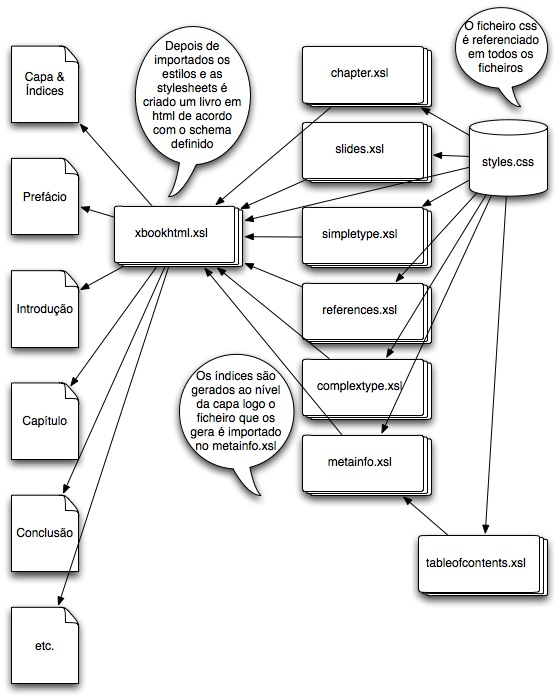
\includegraphics[width=1\textwidth]{./Images/funcspec.jpg}
\caption{Ilustração da especificação funcional do gerador de HTML}
\end{center}
\end{figure}

\hspace{1cm}Para auxílio na construção das páginas e disposição dos vários elementos nas mesmas criamos um ficheiro de estilos utilizando a linguagem \emph{CSS}\useglosentry{glos:CSS}. Esta extensão foi apenas criada para nos dar um maior controlo sobre o resultado final das páginas, para diferenciar os diferentes formatos dos vários elementos e para evidenciar todo o código puramente destinado a alterar o \emph{layout} das páginas, isto é, cores de fundo e de letra, alinhamentos, margens, limites, formatações do texto, etc.

\hspace{1cm}Submetendo um livro escrito de acordo com o \emph{schema} do \emph{XBook} ao gerador de páginas \emph{HTML}\useglosentry{glos:HTML}, vão ser criadas, como resultado, várias
páginas com o conteúdo do livro em separado e com ligação às páginas seguintes hierarquicamente. Certas páginas são criadas obrigatoriamente, como é o caso da capa, à qual é dada o nome do livro em questáo, o prefácio, a introdução, a conclusão e os vários capítulos que compôem o corpo do livro, visto que são obrigatórios de acordo com o \emph{schema} da linguagem. As restantes páginas são criadas apenas caso sejam definidas pelo autor, tal como o índice de tabelas ou imagens.\\

\subsection{\large \emph{Layout} dos Elementos}

\hspace{1cm}Como já foi referido na secção anterior, são criadas páginas para alguns elementos do livro, páginas essas que respeitam uma determinada formatação.
Em todas as páginas o conteúdo encontra-se afastado \emph{2em} (duas vezes o tamanho de letra utilizado) das margens esquerda e direita e \emph{3em} do topo e do fundo.
Todas as páginas, excepto a capa, contêm no topo uma linha horizontal, seguida das hiperligações para os diapositivos adjacentes e de outra linha horizontal para
separá-las do conteúdo.

\hspace{1cm}A capa é dividida em duas partes distintas. A primeira é formada pelo título e subtítulo do respectivo livro, imagem caso exista, informação sobre os vários autores, local de edição, editora e data. No caso de o autor não ter disponível uma imagem, é adicionada uma imagem indicando o mesmo. A segunda parte é constituída pelos vários índices. O índice do conteúdo é apresentado em cascata e permite o acesso a todas as secções do livro através de hiperligações internas ou externas dependendo da localização do elemento de destino. O mesmo se passa em relação aos índices das tabelas e imagens, que apenas diferem na sua imprescindibilidade, visto que apenas são apresentados caso o autor assim o deseje.

\hspace{1cm}As seguintes secções do livro partilham todas o mesmo \emph{layout}, apenas diferindo a apresentação dos diferentes elementos. Os elementos básicos na sua maioria já tinham conversão directa para \emph{HTML}\useglosentry{glos:HTML} por isso não houve muita dificuldade em implementá-los.\\

\begin{small}
\begin{lstlisting}
<xsl:template match="super">
        <sup class="wrap"><xsl:apply-templates/></sup>
</xsl:template>
    
<xsl:template match="sub">
        <sub class="wrap"><xsl:apply-templates/></sub>
</xsl:template>
\end{lstlisting}
\end{small}
\begin{footnotesize}
\begin{center}
\caption{Exemplo do superscript e subscript}
\end{center}
\end{footnotesize}

\hspace{1cm}Também de dificuldade reduzida foi a implementação dos elementos de texto especiais como é o caso das observações, citações ou expressões. Todas elas gozam de particularidades específicas que permitem a sua diferenciação permitindo assim a reprodução do seu comportamento através dos comandos \emph{HTML}\useglosentry{glos:HTML}. Por exemplo as observações são apresentadas numa letra diferente e mais reduzida, alinhada ao centro ao invés das expressões que são apresentadas entre aspas, em itálico, com a mesma letra e tamanho que as observações e inserida no texto.\\

\begin{small}
\begin{lstlisting}  
<xsl:template match="obs">
   <br/><center>
      <p>
         <small><font face="Helvetica"><xsl:apply-templates/></font></small>
      </p>
   <center>
 </xsl:template>

<xsl:template match="exp">
   <em>
      <q>
         <small><font face="Helvetica"><xsl:value-of select="."/></font></small>
      </q>
   </em>
</xsl:template>
\end{lstlisting}
\end{small}
\begin{footnotesize}
\begin{center}
\caption{Implementação das observações e expressões}
\end{center}
\end{footnotesize}

\hspace{1cm}Ao contrário dos casos anteriores, em que os espaços ou alinhamento não tinham importância visto que a \emph{stylesheet} iria adaptar tudo para o formato definido, existem elementos em que faz sentido manter a estrutura e organização definida pelo autor como o caso de apresentações de código. Nestes casos os espaços são respeitados sendo dada a total liberdade ao autor para moldar o resultado final do bloco de código.\\

\begin{small}
\begin{lstlisting}        
<xsl:template match="code">
   <p><code class="space"><xsl:apply-templates/></code></p>
</xsl:template>

<xsl:template match="comment">
   <small>
      <i>
         <font face="Comic Sans">
            <xsl:text> # </xsl:text>
            <xsl:value-of select="."/>
         </font>
      </i>
   </small>
</xsl:template>

.space {white-space: pre} #código css
\end{lstlisting}
\end{small}
\begin{footnotesize}
\begin{center}
\caption{Comportamento no caso de bloco de código}
\end{center}
\end{footnotesize}

\hspace{1cm}Após a parte da apresentação em \emph{slides}, os elementos mais complexos, como a tabela, foram os mais difíceis de implementar e de apresentar na forma de \emph{HTML}\useglosentry{glos:HTML}, apesar de existirem comandos que auxiliem a construção deste tipo de elementos. Elementos como as listas numeradas ou não numeradas são elementos complexos que necessitam de uma aproximação cuidadosa desde a sua especificação no \emph{schema} da linguagem, visto que, apesar do auxílio das comandos de \emph{HTML}\useglosentry{glos:HTML}
são complicados de elaborar devido à possibilidade de recursividade e de ser composta por outros elementos complexos. Podemos então afirmar que a \emph{stylesheet} \emph{complextype.xsl} é a mais complexa e mais elaborada a par da \emph{slides.xsl}.\\
         
\begin{small}                        
\begin{lstlisting}
<xsl:template match="itemize">
    <xsl:choose>
        <xsl:when test="parent::item">
            <ul class="disp">
                <xsl:apply-templates/>
            </ul>
        </xsl:when>
        <xsl:otherwise>
            <ul class="out">
                <xsl:apply-templates/>
            </ul>
        </xsl:otherwise>
    </xsl:choose>
</xsl:template>

<xsl:template match="item">
    <xsl:choose>
        <xsl:when test="itemize or enumeration">
            <xsl:apply-templates/>
        </xsl:when>
        <xsl:otherwise>
            <li><xsl:apply-templates/></li>
        </xsl:otherwise>
    </xsl:choose>
</xsl:template>
\end{lstlisting}
\end{small}
\begin{footnotesize}
\begin{center}
\caption{Listas não numeradas}
\end{center}
\end{footnotesize}

\subsection{\large Principais Decisões e Desafios}

\subsubsection{Index}                           

\hspace{1cm}A primeira grande decisão no caso do gerador de \emph{HTML}\useglosentry{glos:HTML} foi não incluir o elemento \emph{index} visto não fazer muito sentido numa página. Poderíamos ter optado por criar uma página que contivesse todas as palavras que o utilizador quisesse referenciar na secção do \emph{index} e para cada uma dessas palavras criar referências para todas as suas ocorrências no livro. Esta opção não nos pareceu uma solução eficiente e escalável logo decidimos não a incorporar. Claro que não incluir esta página iria criar alguns desafios que iremos esclarecer nas seguintes secções.\\
                        
\subsubsection{Contadores}

\hspace{1cm}Durante o livro existem vários elementos que necessitam que as suas ocorrências sejam contadas, essas contagens podem cobrir o livro por inteiro ou apenas algumas secções. As secções, por exemplo, devem ser diferenciadas entre capítulos, ou seja, cada capítulo deve iniciar um contagem diferente para as suas respectivas secções, o mesmo deve ser feito pelas secções em relação às suas subsecções e assim recursivamente. No caso dos exemplos, tabelas ou figuras já não nos encontramos
perante a mesma situação porque normalmente estes elementos são totalizados ao longo do livro por uma única contagem. Logo temos duas situações distintas que implicam duas implementações distintas.

\hspace{1cm}No caso dos capítulos e seus derivados é apenas necessário utilizar o elemento nativo do \emph{XSL}, \emph{xsl:number} com o parâmetro \emph{count} e depois basta indicar quais os elementos \emph{XBook} sobre os quais queremos actuar e se pretendemos multi-nível (necessário para casos em que sejam definidas subsecções). O código para realizar esta tarefa seria o seguinte:\\

\begin{small}                        
\begin{lstlisting}
<xsl:number count="section|subsection" level="multiple"/>
\end{lstlisting}
\end{small}
\begin{footnotesize}
\begin{center}
\caption{Contagem das secções e subsecções utilizando multi-nível}
\end{center}
\end{footnotesize}

\hspace{1cm}O outro caso é relativamente mais complicado devido ao facto de não podermos usar o elemento \emph{xsl:number} como no caso anterior, dado que apenas contaria os elementos que derivassem do que nós desejávamos totalizar (inclusive). A forma mais eficaz que nos ocorreu na altura foi, contar todos os elementos iguais em tipo que já tinham sido processados e consequentemente ultrapassados. Para efectuar esta operação tivemos que recorrer a expressões \emph{XPath}, que nos
possibilitaram recuar na travessia e contar tudo o que já tinha sido processado para três. Antes de tudo é necessário declarar uma variável que assuma o valor de todos os elementos desejados que se encontrem para três, posteriormente é necessário seleccionar o valor dessa variável e somar um para igualar a posição do elemento actual e apresentando-o no local pretendido.\\
         
\begin{small}                        
\begin{lstlisting}
<xsl:template match="fig">
    <xsl:if test="@label">
        <a name="{@label}"/>
    </xsl:if>
    <a name="{generate-id(.)}"/>
    <xsl:variable name="fg" select="count(preceding::fig)"/>
    <br/><center><p>
        <xsl:apply-templates select="img"/>
        <small><p>
            <xsl:text>Fig. </xsl:text>
            <xsl:value-of select="$fg+1"/>
            <xsl:text>: </xsl:text>
            <xsl:apply-templates select="caption"/>
        </p></small>
    </p></center>
</xsl:template>
\end{lstlisting}
\end{small}
\begin{footnotesize}
\begin{center}
\caption{Exemplo do \emph{template} da figura}
\end{center}
\end{footnotesize}

\subsubsection{Capítulos}

\hspace{1cm}Os capítulos foram uma das maiores fontes de problemas devido ao facto de ser um dos componentes maioritórios da estrutura de um livro e ser o único desses que não é filho do elemento raíz do \emph{XBook}, isto é, todos os outros elementos principais têm como pai o elemento \emph{xbook} excepto os capítulos que têm como pai o corpo do livro (\emph{body}). Embora isto não parece minimamente significativo, levou a elaboração de várias linhas de código para contornar esta divergência.

\hspace{1cm}Considerando o caso em que queremos criar uma referência para uma figura contida na conclusão, é apenas necessário seleccionar, através de expressões \emph{XPath}, os antepassados dessa figura e seleccionar o penúltimo deles, neste caso a conclusão. Se por razão alguma a figura passasse para dentro de uma secção de um determinado capítulo esta operação deixaria de funcionar visto que o capítulo não seria o penúltimo antepassado da figura e juntando o facto de não ser gerada nenhuma página \emph{HTML}\useglosentry{glos:HTML} para corpo do livro, este sim o penúltimo antepassado da figura. Outro caso em que está latente a influência dos capítulos nas decisões por nós tomadas é a criação das referências para simular o efeito de diapositivos que permitem ligar todas as páginas entre si, sendo possível aceder a qualquer parte do livro através dessas hiperligações. Mais uma vez todas as páginas criadas são filhos do elemento \emph{xbook} excepto os capítulos, herdando também aqui o problema anterior. Para ligar as páginas entre capítulos a melhor solução seria trabalhar os capítulos como se não existissem outros elementos para além deles e depois apenas os elementos das extremidades se preocupariam em procurar outros elementos para além deles, quase como se funcionasse como uma rede \emph{MPLS}. Deste modo o problema visto pelo lado dos capítulos estava resolvido, mas no caso dos elementos que se encontrem adjacentes ao \emph{body} continuava tudo na mesma visto que continuavam a efectuar a mesma operação que os restantes, isto é, apontar para o seu precedente ou posterior que se encontre no mesmo nível. Para resolver esta situação é necessário criar condições do lado dos elementos filhos do \emph{xbook} para verificar se o elemento precedente ou posterior é o corpo (\emph{body}). É devido à natureza destes desafios que classificamos os capítulos como uma das maiores fontes de problemas deste projecto.\\
  
\begin{footnotesize}
\begin{lstlisting}
<xsl:choose>
    <xsl:when test="preceding-sibling::chapter">
        <xsl:variable name="pre" select="preceding-sibling::chapter/title"/>
        <td align="left" class="linkleft">
           <a href="{$pre}.HTML"><xsl:value-of select="$pre"/></a>
        </td>
    </xsl:when>
    <xsl:otherwise>
        <xsl:variable name="pre" select="ancestor::*/body/preceding-sibling::*[1]/title"/>
        <td align="left" class="linkleft">
           <a href="{$pre}.HTML"><xsl:value-of select="$pre"/></a>
        </td>
    </xsl:otherwise>
</xsl:choose>
\end{lstlisting}
\begin{center}
\caption{Condição para criar hiperligações entre capítulos}
\end{center}
\end{footnotesize}

\subsubsection{Referências}

\hspace{1cm}As referências são sempre um ponto importante em qualquer página, por isso foi necessário algum cuidado para garantir que funcionavam devidamente, isto mais porque o modo de apresentação por diapositivos força a que haja ligações a elementos externos contidos noutras páginas. São possíveis cinco tipos de referências, tabelas, figuras, capítulos, secções ou subsecções e exemplos, destas apenas para os capítulos é criada uma página por isso faz desta referência a mais fácil de
resolver, todos as outras podem ser referências internas ou externas, mas para diminuir as linhas de código necessárias para fazer essa diferenciação, vamos assumir que são todas externas. Para nos referirmos a qualquer elemento, criamos uma ligação que unifica o caminho do ficheiro que o contêm com o endereço interno do próprio. O resultado é algo deste género:\\

\begin{small}                        
\begin{lstlisting}
<a href="{ancestor::*[last()-2]/title}.HTML#{$fig}"><xsl:value-of select="$fig"/></a>
\end{lstlisting}
\end{small}
\begin{footnotesize}
\begin{center}
\caption{Exemplo do código da hiperligação}
\end{center}
\end{footnotesize}

\hspace{1cm}Através deste processo podemos criar uma hiperligação para qualquer elemento do livro que tenha uma etiqueta associada. Claro está que para conseguirmos criar uma hiperligação para qualquer elemento temos que conseguir de algum modo determinar o nome do ficheiro onde se encontra o elemento. Como já tínhamos referido, no caso do capítulo é intuitivo, no caso da secção também é fácil dado que sabemos que fará sempre parte de um capítulo. Apenas as tabelas, figuras e exemplos se podem encontrar em qualquer parte do livro. Como referimos na secção anterior, só são criadas páginas para os elementos filho do \emph{xbook} e para os capítulos logo apenas temos de verificar se o elemento deriva de um capítulo. Podemos verifica-lo da seguinte forma:\\

\begin{footnotesize}                        
\begin{lstlisting}
<xsl:choose>
    <xsl:when test="ancestor::*/chapter">
        <a href="{ancestor::*[last()-2]/title}.HTML#{$ref}"><xsl:value-of select="$ref"/></a>
    </xsl:when>
    <xsl:otherwise>
        <a href="{ancestor::*[last()-1]/title}.HTML#{$ref}"><xsl:value-of select="$ref"/></a>
    </xsl:otherwise>
</xsl:choose>
\end{lstlisting}
\begin{center}
\caption{Implementação da verificação do capítulo como antecessor}
\end{center}
\end{footnotesize}

\subsubsection{Diapositivos}

\hspace{1cm}Possivelmente esta terá sido a tarefa mais complexa e mais complicada do gerador de \emph{HTML}\useglosentry{glos:HTML}, não pelas suas caracterásticas iniciais, mas sim pelas nossas pretensões para este processo. Já foi demonstrado posteriormente que os capítulos influenciavam este processo por isso não o iremos voltar a referir. Como os capítulos, também o \emph{index} afectou o desenvolvimento dos diapositivos devido ao facto de não ter sido incluído na transformação para \emph{HTML}\useglosentry{glos:HTML}, mas ainda assim poder fazer parte do livro. Este problema duplicou o código desenvolvido devido ao facto de termos de criar uma condição especial para verificarmos a presença do \emph{index}. Os \emph{slides} poderiam ter um código muito mais reduzido mas nós pretendíamos garantir uma caracterástica importante que era um factor determinante em futuras alterações do código ou do \emph{schema} da linguagem. Esse factor baseia-se em escrever um algoritmo que permitisse que fossem adicionados novos elementos há actual disposição do \emph{schema} sem que fosse necessário alterar o código da geração das hiperligações que simule o efeito de diapositivos. Para isso foi necessário abstrairmo-nos da disposição dos elementos no \emph{schema} e debruçarmo-nos apenas sobre uma solução que garantisse a possibilidade de criar as ligações independentemente dos elementos do \emph{schema}. A solução à qual chegamos abrange três tipos de casos, o elemento encontrar-se dentro de um capítulo, o nome da página estar armazenada num atributo ou num elemento e a possibilidade de presença do \emph{index}, e cumpre os requisitos que determinamos, a possibilidade de alterar o \emph{schema} sem implicar ter de alterar o código.\\

\subsubsection{índices}

\hspace{1cm}No elemento \emph{xbook} são definidas três atributos, um obrigatório e dois opcionais. O índice de conteúdos é obrigatório e o das tabelas e figuras são opcionais dando a possibilidade de o autor optar por introduzir todos ou apenas um índice, conforme o desejar. Para criar os índices das tabelas e figuras é apenas necessário acoplar os vários processos sugeridos anteriormente para obtermos o efeito desejado. Os maiores desafios destes dois tipos de índice é contar o
número de elementos do tipo já processados e encontrar a sua localização absoluta no livro. Ambas os desafios já foram resolvidos anteriormente por isso bastaria uni-los e definir o \emph{layout} desejado. Para o índice de conteúdos teríamos que processar novamente todos os elementos principais de modo a angariar toda a informação necessária para o construir, no entanto nós já tínhamos um \emph{template} para cada elemento o que nos impedia de o voltar a fazer, pelo menos do mesmo
modo, logo fomos forçados a criar um novo modo de travessia ao qual chamamos \emph{indice}. Este modo permitiu-nos efectuar a travessia através de novos \emph{templates} definidos para este caso em concreto. Visto que no índice apenas aparecem os elementos filho do \emph{xbook}, capítulos, secções e subsecções foi praticamente imediata a resolução dos endereços para as várias páginas, apenas residindo alguma dificuldade na resolução das hiperligações para as secções e subsecções visto serem as únicas para às quais não são criadas páginas \emph{HTML}\useglosentry{glos:HTML} próprias. Apesar desse factor, esta tarefa é de fácil resolução devido ao facto de já ter sido resolvida posteriormente na secção das referências.\\

\subsubsection{CSS}

\hspace{1cm}Finalmente, optêmos por elaborar num ficheiro à parte todos os estilos de formatação, alinhamento, etc., para melhorar a legibilidade e diminuir as linhas de código nas \emph{stylesheets} e pôr em evidência e organizar todo o código \emph{CSS}\useglosentry{glos:CSS}. Este aspecto não foi um desafio, apenas uma decisão tomada devido aos factores aqui apresentados. Para permitir ao \emph{browser} encontrar o ficheiro é necessário associar o \emph{CSS}\useglosentry{glos:CSS} aos ficheiros \emph{HTML}\useglosentry{glos:HTML} gerados através da
inserção da linha abaixo apresentada no cabeçalho da estrutura \emph{HTML}\useglosentry{glos:HTML}.\\

\begin{small}                        
\begin{lstlisting}
<link XMLns="http://www.w3.org/1999/xHTML" type="text/css" href="styles.css"/>
\end{lstlisting}
\end{small}

\newpage

%%
% Secção
%%
\section{\LARGE Oxygen Author}

\hspace{1cm}O \emph{Author} é uma ferramenta útil para os utilizadores que não se sentem à vontade para redigir o seu livro em \emph{xml} e também para facilitar de um certo modo a elaboração do livro. Não é preciso ter conhecimentos de \emph{xml} para escrever um livro na versão do \emph{XBook Author}. Os elementos assumem comportamentos no \emph{Author} exactamente iguais aos adoptados na geração do documento em formato \emph{pdf}, devido à utilização da linguagem \emph{CSS}, que contêm
a maioria dos comandos ou funções utilizadas no \emph{XSL:FO}.

\hspace{1cm}Visto que já nos referimos anteriormente a \emph{CSS} neste relatório e que a maioria dos código apenas serve para alterar o \emph{layout} do documento, nesta secção vamos apenas discutir as novas funções e fazer uma comparação com algumas expressões de \emph{XSL} e \emph{XPath}.
                
\hspace{1cm}Ao longo da realização desta tarefa, verificamos que o código \emph{CSS} se assemelhava ao \emph{XSL:FO} em termos sintácticos e que também partilhava algumas semelhanças semânticas com o \emph{XSL}, semelhanças essas que permitiram que nós efectuássemos todas as operações necessárias para uma eficiente e organizada apresentação de um livro. As expressões \emph{CSS} que utilizamos para realizar esta tarefa são apresentadas em seguida:\\

\begin{itemize}
        \item \emph{child} $\rightarrow$ A expressão \emph{child} de \emph{XPath} é representada pelo símbolo '$>$', a sua existência permite-nos aplicar estilos aos filhos de respectivos elementos, possibilitando a diferenciação em relação a outros elementos com o mesmo nome. No exemplo escolhido são aplicadas algumas formatações aos filhos \emph{caption} do elemento \emph{fig}, não abrangendo assim as legendas das tabelas.\\
        
        \begin{small}
        \begin{lstlisting}
        fig > caption{
            display:table-caption;
            font-size:small;
            text-align:center;
}
        \end{lstlisting}
        \end{small}
        
        \item \emph{following-sibling} $\rightarrow$ O símbolo '+' tem o mesmo comportamento que o \emph{following-sibling} em \emph{XSL}, e foi através dele que conseguimos implementar os contadores nas secções e subsecções. No exemplo seguinte, sempre que uma subsecção fosse precedida por um bloco de texto, era inicializada um contador denominado \emph{subsec}.\\
             
        \begin{small}
        \begin{lstlisting}
        textblock + subsection{
            counter-reset:subsec;
}
        \end{lstlisting}
        \end{small}
        
        \item \emph{descendant} $\rightarrow$ No caso da expressão \emph{descendant}, a expressão proporcional é um elemento seguido de outro separados por um espaço. No seguinte exemplo, para todos os elementos \emph{exercise} descendentes de \emph{exercises}, o contador \emph{exec} é incrementado e é impresso para o documento, utilizando o '.' como separador multi-nível.\\
        
        \begin{small}
        \begin{lstlisting}
        exercises exercise{
            display:block;
            counter-increment:exec;
            content:counters(exec,".")") ";
}
        \end{lstlisting}
        \end{small}
\end{itemize}                            
                        
\subsection{Atributos}

\hspace{1cm}A utilização dos atributos e possíveis condições conforme a existência ou valor de um atributo foi outra boa surpresa nesta linguagem. Através da utilização de atributos foi-nos possível introduzir no \emph{template} visto pelo utilizador os valores das \emph{urls} definidas pelo mesmo.\\

\begin{small}
\begin{lstlisting}
img{
    display:block;
    text-align:center;
    content:attr(path,url);
}
\end{lstlisting}
\end{small}

\hspace{1cm}O comando \emph{attr} permite-nos invocar os atributos do elemento onde nos encontramos. Também podemos verificar se um elemento existe através da expressão \emph{elemento[atributo]}.\\

\subsection{\emph{After} e \emph{before}}

\hspace{1cm}Podemos alegar que estes foram duas das expressões mais úteis que utilizamos na realização do editor para o \emph{Author}, devido à sua extrema utilidade. As expressões \emph{after} e \emph{before} permitem efectuar operações antes e depois de processar um determinado elemento, respectivamente. Por exemplo, ao apresentar uma referência desejávamos que ela aparece-se entre chavetas, para conseguirmos este efeito apenas necessitávamos de processar a chaveta antes e depois de
processar uma referência. O código para obter o efeito é o seguinte:\\
       
\begin{small}
\begin{lstlisting} 
tabref,figref,secref,chpref,exref{
    display:inline;
    font-style:oblique;
}

tabref:before,figref:before,secref:before,chpref:before,exref:before{
    content:"{";
}

tabref:after,figref:after,secref:after,chpref:after,exref:after{
    content:"}";
}
\end{lstlisting}
\end{small}

\subsection{Contadores}

\hspace{1cm}Para concluir, apresentamos o ponto mais difícil de realizar aquando a realização do editor para o \emph{Author}. Isto deve-se ao facto de os contadores funcionarem de modo diferente em relação a \emph{XSL}. Existem dois tipos de contadores, o \emph{counter} e o \emph{counters}. O \emph{counter} é equivalente à expressão \emph{xsl:number count="[element]" level=single}, e o \emph{counters} é relativamente semelhante à mesma expressão, apenas alterando o nível para múltiplo. Na função \emph{counters} é também possível definir o separador desejado para intercalar os caracteres do contador, normalmente números.\\

\begin{small}
\begin{lstlisting}
xbook{
    display:block;
    margin:2em;
    counter-reset:tab fig exm;
}
\end{lstlisting}
\end{small}

A função \emph{counter} tem algumas variantes que permitem controlar da melhor forma os contadores. No exemplo acima, são inicializadas três variáveis através da função \emph{counter-reset}, que irão totalizar o número de tabelas, figuras e exemplos, respectivamente.

\hspace{1cm}No exemplo seguinte, são contados os números de capítulos através da função \emph{counter-increment} e também é inicializada a varíavel que tem como objectivo contar o número de secções do respectivo capítulo.\\

\begin{small}
\begin{lstlisting}
chapter{
    display:block;
    padding-top:1em;
    padding-bottom:1em;
    counter-increment:chp;
    counter-reset:sec;
}
\end{lstlisting}
\end{small}

\hspace{1cm}Após termos abordado as principais variantes da função \emph{counter}, podemos implementar o contador mais trabalhoso e complicado, o das subsecções. A implementação é apresentada no exemplo abaixo.

\begin{small}
\begin{lstlisting}
section > title:before{
    counter-increment:sec;
    content:counter(sec)". ";
    counter-reset:subsec;
}

subsection > title:before{
    counter-increment:subsec;
    content:counter(sec)"."counters(subsec,".")" ";
}

textblock + subsection{
    counter-reset:subsec;
}
\end{lstlisting}
\end{small}

\hspace{1cm}Antes de tudo ao encontrarmos uma secção, e antes de imprimirmos o título, incrementamos o contador das secções \emph{(sec)} visto que nos encontramos a processar uma secção. Depois imprimimos o valor do contador para aparecer à frente do título, e inicializamos uma nova varíavel \emph{(subsec)} que vai contar o número de subsecções incluídas na actual secção. Posteriormente, nas subsecções é necessário incrementar o contador das subsecções visto nos encontrarmos numa, e imprimimos o número da actual secção seguido do contador multi-nível das subsecções. Estas condições por si só não são suficientes dado que é necessário iniciar um novo contador sempre que se encontrar subsecções embutidas em subsecções. Para garantir a criação da varíavel, sempre que uma subsecção suceder a um bloco de texto deve-se iniciar um novo contador, isto porque a primeira subsecção de uma subsecção sucede sempre um bloco de texto, ou seja, uma condição que será sempre satisfeita.

\newpage

%%
% Secção - Testes e Resultados
%%
\newpage
\section{\LARGE Resultados Obtidos}
\hspace{1cm}Para evitar que o utilizador esteja a editar o ficheiro XML sempre que quer alterar o conteúdo do seu documento, decidimos criar um editor como mostramos na secção anterior. Se utilizarmos um dos ficheiros testes que disponibilizamos, e o carregarmos para o nosso editor de XML, vamos verificar que podemos fazer qualquer tipo de alteração ao documento sem termos a noção do código {\em XML}\useglosentry{glos:XML} que está por trás. A numeração das secções, figuras, tabelas, etc., é feita automaticamente pelo editor.

\hspace{1cm}Podemos agora converter o nosso documento para {\em PDF}\useglosentry{glos:PDF} de forma a ficarmos com um documento que segue o formato de um livro ({\em stylesheet exemploPDF.xsl}). Ou então se preferirmos podemos criar uma página {\em HTML}\useglosentry{glos:HTML} ({\em stylesheet xbookHTML.xsl}) com fácil acesso às várias secções do livro, com o uso de {\em links}.\\

%%
% Secção - Conclusão
%%

%Síntese / Recapitulação do Relatório
%Resultado Atingido / Crítica
%Trabalho Futuro

\newpage
\section{\LARGE Conclusão}
\hspace{1cm}Durante o relatório vimos que existem várias formas de definir os mesmos elementos no \verb|schema| e que estas podem ter um peso considerável a dificuldade no desenvolvimento das {\em stylesheets}. Podemos então dizer que a construção do \verb|schema| tem que ser feita de uma forma pensada tendo também em conta facilitar o desenvolvimento das aplicações que nele se vão basear.

\hspace{1cm}Conseguimos chegar a uma boa base para um trabalho futuro mais exaustivo e, sabemos que este projecto ainda apresenta algumas limitações mas estamos à espera de resolver algumas de forma a diminuir a complexidade de implementação e tornar o este projecto o mais escalável possível.

\hspace{1cm}Sabemos que a forma como definimos as listas no \verb|schema|, tornaram muito mais complexa a forma como as convertemos para {\em PDF}\useglosentry{glos:PDF} ou para {\em HTML}\useglosentry{glos:HTML}.

\hspace{1cm}Sabemos que há elementos que ficaram por definir, e por isso estamos a pensar acrescentar mais alguns ao nosso \verb|schema| (como por exemplo as notas de rodapé). Tencionamos transformar o elemento dos anexos numa lista de secções de forma a permitir vários anexos ordenados por ordem alfabética.

\hspace{1cm}Depois de desenvolvidas as {\em stylesheets} percebemos que nos daria mais jeito as referências serem atributos ao invés de elementos, por isso essa também será algo a alterar no nosso \verb|schema|.

\hspace{1cm}Na conversão de {\em XML}\useglosentry{glos:XML} para {\em PDF}\useglosentry{glos:PDF}, tencionamos implementar o index e alterar a forma como a página de cada capítulo é impressa, acrescentando a informação de um subtítulo caso este exista.

\hspace{1cm}Ao gerar as páginas {\em HTML}\useglosentry{glos:HTML} pensamos que será melhor ao gerar o nome das páginas utilizar o {\em generate-id} em vez de atribuirmos o nome como identificador, isto para evitar ambiguidades.

\hspace{1cm}Quanto ao nosso editor, as únicas alterações que tencionamos fazer são aquelas que fizermos no nosso \verb|schema|, já que só dele depende.\\

\newpage
\printglossary
\addcontentsline{toc}{section}{\LARGE Glossary}

\end{document}